\chapter{Distributed control system}
\begin{overview}
The different data acquisition architectures are discussed in this chapter and the implementation of a control system using in the Simulink environment is shown. The location of the different software components are also given. 
\end{overview}

\section{Distributed data acquisition and control}
A schematic of the different \eindex{distributed control systems} that can be implemented in the process control laboratory is shown in figures~\ref{fig:control:ddcs} to ~\ref{fig:control:clust}. 
\begin{figure}[htbp]
  \centering
  \subfigure[Distributed digital control system]{
  	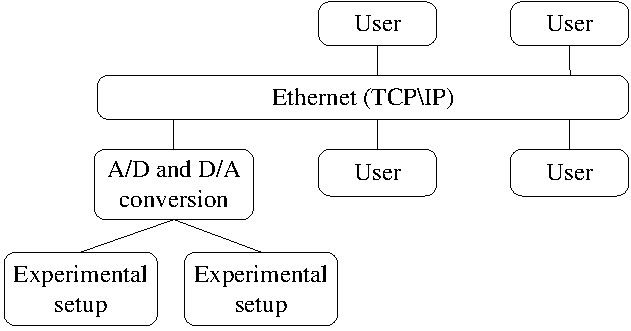
\includegraphics[width=0.6\textwidth]{controlddcs}
  	\label{fig:control:ddcs}
  }  
  \subfigure[Supervisory digital control system]{
  	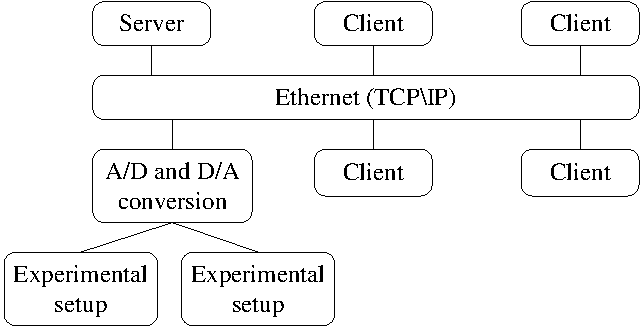
\includegraphics[width=0.6\textwidth]{controlscada}
  	\label{fig:control:scada}
  }
  \subfigure[Clustered supervisory control system]{
  	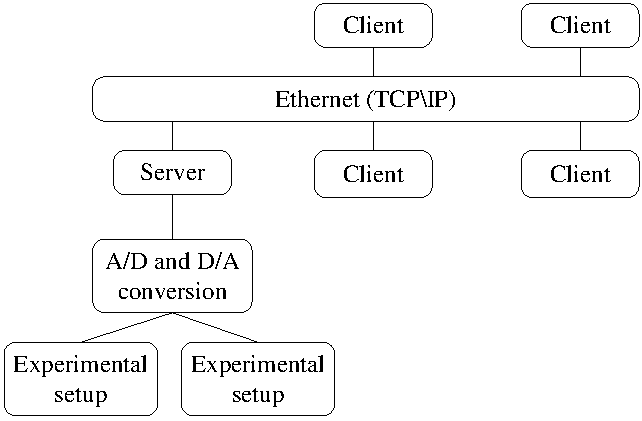
\includegraphics[width=0.6\textwidth]{controlclust}
  	\label{fig:control:clust}
  }
 	\caption{Different digital control configurations}
\end{figure}

The analog measurements is converted to a digital signal and is sent across the ethernet using the \eindex{TCP/IP} format, which is a well accepted protocol defined specifically for use with the ethernet. The control signals originating from the computers connected to the ethernet is converted back to a analog signal and sent to the actuators of the process. The different architectures regarding the interaction of the different computers on the ethernet is subsequently discussed.

\begin{description}
	\item [Distributed data acquisition and control]. The analog measurements are sent directly to the user computers through the ethernet connection and the process receives the digital control signal from the user computer via the same route. 
	
A great advantage of this approach is that any user can be used for the control of any unit should one user fail, but data integrity is at risk as there is no central data archiving device. The user computer is therefore responsible for both data acquisition and control, hence the name \eindex{distributed data acquisition and control}.   

\item[Supervisory data acquisition and control] A server is placed on the ethernet highway for the control configuration, and is responsible to give access to the different users or clients of the control system, store the data and check the  variables for alarm management. 

The fact that the clients must log onto the server before the control system can be used gives greater security and control over the different experimental setups. 

\item[Clustered supervisory data acquisition and control] The server is connected directly to the A/D and D/A instrumentation. This increases data integrity as the data to the server is not transmitted of the ethernet connection. The \eindex{bandwidth} (indication of ethernet use) of the ethernet is also reduced.
\end{description}

\section{Software and communication protocols}
The different software used (and their interaction) for the control of the experimental setups is shown in figure~\ref{fig:control:soft}. The schematic shows that there are two ways or routes to communicate with the experimental setups from Simulink, which is the software used to implement the control algorithms in the process control laboratory. 
\begin{figure}[htbp]
	\centering
	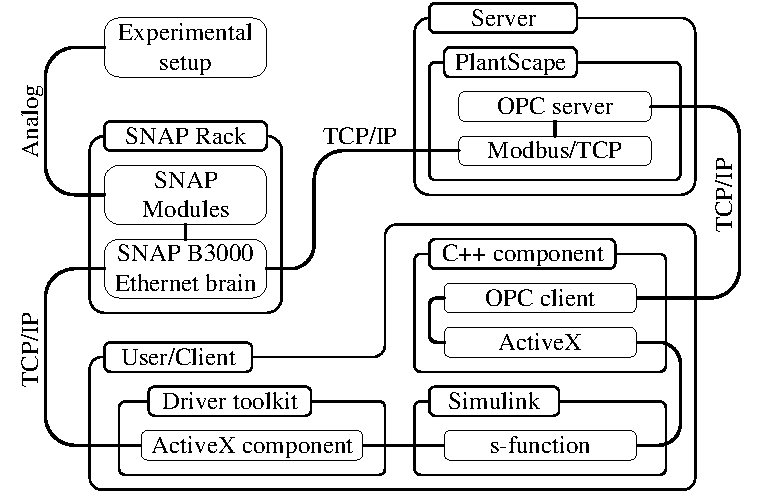
\includegraphics[width = 0.7\textwidth]{controlsoft}
	\caption{Software protocols used}
	\label{fig:control:soft}
\end{figure}

The first route can be with the use of the \eindex{driver toolkit} from OPTO22 that utilises \eindex{ActiveX}, which is a protocol defined for interfacing different software programs in the Windows environment, to communicate directly with the A/D and D/A conversion devices (SNAP B3000 brain, etc.).

The second route is with the use of a server and specific \eindex{SCADA} (Supervisory Control and Data Acquisition) software that uses \eindex{MODBUS/TCP}, a protocol defined for instrument interfacing over a ethernet connection, to communicate with the A/D and D/A conversion devices. A custom \eindex{C++ component} was developed in-house to enable \index{Simulink} that utilises \eindex{ActiveX} to communicate with the server using \eindex{OPC}, another control protocol defined for inter controller communication via ethernet connections.

Figure~\ref{fig:control:soft} shows further that the \eindex{Driver Toolkit} and the \eindex{C++ component library} must be installed on the user or client computer. The software can be found on $\backslash$$\backslash$groa$\backslash$lab$\backslash$Opto for the \eindex{Driver Toolkit} and $\backslash$$\backslash$groa$\backslash$lab$\backslash$PlantStar fot the \eindex{C++ component library}.

The s--function needed for the interfacing of \eindex{Simulink} with the experimental setups can be obtained from $\backslash$$\backslash$groa$\backslash$lab$\backslash$Rigs. More information on the development of the s--function can be obtained from the in--house \emph{Matlab Opto22 driver manual}.

The \eindex{Real time clock} block is used to force the \eindex{Simulink} simulation to run at real time and must therefore be included on the model of the control algorithm used for control. The block icon can be seen in figure~\ref{fig:control:clock}. The s--function and model of the \eindex{real time clock} can be found at $\backslash$$\backslash$groa$\backslash$lab$\backslash$Matlab$\backslash$Rtclock and must be included in the current \emph{Matlab} path to run.
\begin{figure}[htbp]
	\centering
	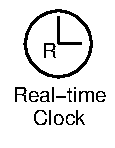
\includegraphics[width = 0.1\textwidth]{controlclock}
	\caption{Real time clock icon}
	\label{fig:control:clock}
\end{figure} 

\begin{example}
The of the s--function block using the ActiveX component \index{ActiveX component} calls for the level and flow control loop can be seen in figure~\ref{fig:control:sfunc}, and shows that two inputs for the control valves (4--20 mA) and two outputs (-20--20 mA) for the liquid level and liquid flow are available for the implementation of a control algorithm.
\begin{figure}[htbp]
	\centering
	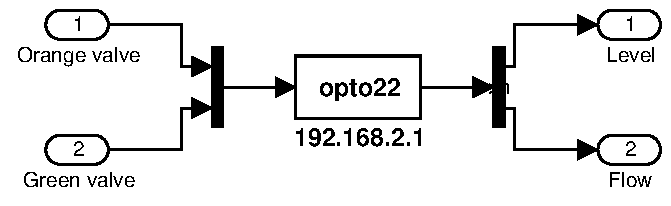
\includegraphics[width = 0.5\textwidth]{controlsfunc}
	\caption{s--function implementation of the level and flow model}
	\label{fig:control:sfunc}
\end{figure}

%An implementation of a PID controller for the tank level of the flow control loop can  be seen in figure~\ref{fig:control:model}. The one control input and the flow output is zeroed as it is not used for the current control implementation.
%\begin{figure}[htbp]
%	\centering
%	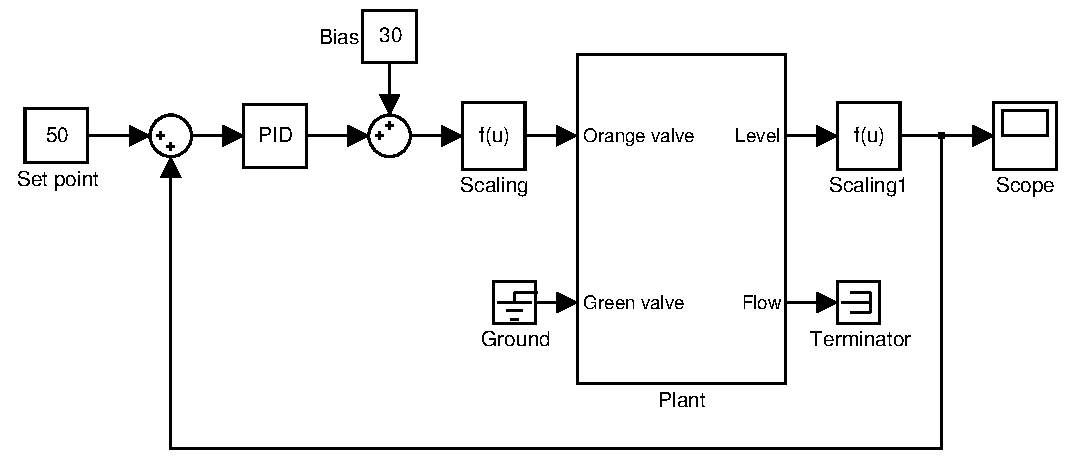
\includegraphics[width = 0.8\textwidth]{controlmodel}
%	\caption{Single loop control of the tank level}
%	\label{fig:control:model}
%\end{figure}
\end{example}
	  